\chapter{Combining Graph Kernels Efficiently}
\label{Chapter3}

This chapter details the contribution of the present work.
We discuss in detail the proposed methodology (Section \ref{sec:meth}) and
finally give an overview of the main optimization choices (Sections
\ref{sec:opt}, and \ref{sec:inc})

\section{Proposed methodology}
\label{sec:meth}
%thorough description

Having discussed the need for kernels combination and the possible techniques
available in the literature, we now proceed to illustrate the main idea behind
the present work.

As discussed in Section \ref{subsec:mkl}, $MKL$ methods generally provide a consistent
way of using different, possibly weak, kernels to build a model which is the result
of their composition in some way that vary from implementation to implementation.
The constant point here is that the set of weak kernels gets \emph{combined}, thus
making one of those methods the perfect candidate to be the foundation of our
combining methodology.

The easyMKL implementation (Section \ref{subsec:easymkl}) was deemed a good
choice because of the promising overall performances and the empirical evidence
that the method is not significantly affected by the number of kernels
being combined, a major point of our method, and last but not least it was
available and easily integrated with our pre-existing kernels code base.

The methodology therefore consists in a k-fold nested cross-validation with
easyMKL as the kernel machine as detailed in Algorithm \ref{alg:method} and further in
Figure \ref{fig:method}.

\begin{algorithm}
    \caption{
        High level implementation of the proposed methodology.
        The $computeKernel$ function returns a kernel matrix computed
        according to the selected $kernel$ from the $Kernels$ set which indexes
        the kernels to be combined, the hyper-parameters $tuple$ and the chosen
        $dataset$.
        The $split$ function takes a list of kernel matrices and returns two lists
        of kernel matrices split in two sets according to the cross-validation
        strategy and the $Folds$.
        The $easyMKL$ function takes a $\Lambda$ parameter and a list of kernel
        matrices to return a $model$.
    }
    \label{alg:method}
    \begin{algorithmic}[1]
        \State $K \gets []$
        \Comment{K is the list of kernel matrices}
        \label{line:kernels}
        \ForAll{$kernel \in Kernels$}
            \ForAll{$tuple \in paramsgrid$}
                \State $K_{kernel} \gets \Call{computeKernel}{kernel, tuple, dataset}$
            \EndFor
        \EndFor

        \ForAll{$outerfold \in Folds$}
            \State $trainingset, testset \gets \Call{split}{K, outerfold}$
            \label{line:osubsets}
            \ForAll{$\Lambda \in params$}
                \ForAll{$innerfold \in Folds$}
                    \State $trset, validationset \gets \Call{split}{trainingset, innerfold}$
                    \label{line:isubsets}
                    \State $model \gets \Call{easyMKL}{\Lambda,trset}$
                    \State validate $model$ with $validationset$
                \EndFor
            \EndFor
            
            \State select the best $(model,\Lambda)$ resulting from the inner loop
            \State $finalmodel \gets \Call{easyMKL}{\Lambda,trainingset}$
            \State test $finalmodel$ with $testset$
        \EndFor

        \State \Return $finalmodel$ with best average among the $Folds$
    \end{algorithmic}
\end{algorithm}

\begin{figure}[ht]
    \centering
    \includegraphics[scale=0.5]{Figures/nested}
    \caption{The method illustrated. First the dataset, composed of a list of
    kernel matrices get split into a training set and a test set (1).
    Then a $k$-fold cross-validation is performed on the training set ($k$ was set to
    10 in our case) (2) and the best resulting model is selected according to some
    performance measure (3). The selected model gets re-trained on the whole initial
    training set (4) and finally gets tested against the test set that was left out
    during the entire process (5). At the end of the outer loop of the nested
    cross-validation, the best model is again selected according to the chosen
    metric (6).}
    \label{fig:method}
\end{figure}

The code is divided in two parts: first we have the kernel computation phase,
in which we take the parameters grid and compute all the kernel matrices for each
parameters tuple, for each kernel to be combined.
The second part consist in the two loops of the nested cross-validation, see
Section \ref{subsubsec:ncv} for details.

The new idea behind an otherwise standard and tried scheme of operations is that
the kernel list instantiated in line \ref{line:kernels}, comprises all the 
kernels computed from the grid of parameters combinations that would otherwise
have been individually fed to a standard single kernel machine (e.g. SVM).
Doing so, the single kernel hyper-parameter optimization phase can be avoided in its
entirety and the only parameters that needs validation are the ones of the chosen
$MKL$ implementation, namely one regularization parameter ($\Lambda$) in our case.
This point will be further elaborated on in the following section.

\subsection{Embedded model selection}
\label{subsec:parameters}
One of the main advantages of the proposed method is that it permits to embed
the otherwise cumbersome process of hyper-parameter optimization (Section \ref{subsubsec:grid})
inside the learning phase in a completely transparent way, which will be hereby
described.

It is customary practice to perform hyper-parameter optimization employing a grid
search technique.
In our setting this would translate to having to compute one kernel matrix
for all the possible combinations deriving from every set of values
chosen for each kernel hyper-parameter, and repeat the process for every kernel
we may have wanted to combine.
Then a cross-validation would have been performed using a kernel matrix from each
selected kernel, according to a combination of parameters.
Let the kernel be the $ODDK_{ST}$, its parameters be $h$, $\lambda$ and let $\Lambda$
be the hyper-parameter of easyMKL; if we let $l,m,n$ be the cardinalities of the three
sets of values respectively, the cross-validation instances would have been $l\cdot m\cdot n$.

A first improvement over the above scenario is to adopt another $MKL$ approach 
and give the algorithm the kernels matrices computed from the grid all at once.
With the above described settings we are reducing the number of needed
cross-validation instances from $l\cdot m\cdot n$ to $n$, hence potentially
reducing the size of the whole process by orders of magnitude.
A visual comparison of these two approaches is given in Figure \ref{fig:comparison}.

\begin{figure}[ht]
    \centering
    \includegraphics[scale=0.6]{Figures/comparison}
    \caption{Comparison between the standard approach (A) and the proposed one (B).
    $K_1,\dots,K_N$ refers to the $N$ kernels computed from the $N$ combinations
    derived from the parameters grid. In (A) each kernel is used to perform a full learning
    cycle, $N$ in total. On the other hand in (B), the $N$ kernels all together are
    given as input to the only one learning cycle to be performed. The kernel machines
    in the diagrams has been instantiated to the ones chosen in this study.}
    \label{fig:comparison}
\end{figure}

Another advantage of this approach is that instead of selecting one combination
of parameters thus restricting the generalization power of the resulting model,
the whole set of parameters combination concurs in the model determination hence
increasing the chances of it being more general while boosting the overall performances
of the single kernels.

Given the fact that our $MKL$ implementation of choice has an algorithmic
complexity that is not dependent on the cardinality of the input but rather on
its dimensions, it can be easily be the case that hundreds of kernel are used
at once; this can lead to an increase of the memory consumption in a measure
proportional to the size of the input dataset.

Section \ref{sec:opt} deals with a possible algorithmic solution to this problem,
while the following section will show how it is possible to combine the idea here
described with another technique used in multiple kernel learning to further
improve the feature spaces and reduce the computational burden and space
requirements eliminating one hyper-parameter.

\subsection{Kernels and feature spaces}
\label{subsec:features}

Even if in principle $MKL$ algorithms can deal with large number of kernels, the
memory consumption problem previously described will manifest itself even for
datasets of modest dimension, depending on the parameters grid.

Beside adopting a sampling strategy on the dataset, thus reducing the dimension
of the kernel matrices while sacrificing some learning potential, another
solution consist in reducing the number of hyper-parameters that concur
in generating the parameter grid which size will directly determine the number
of total kernels to combine.

In this study we were working with graph kernels and this fact allowed us to employ
the feature division strategy delineated in \cite{gmkl} where applicable and similarly
devise a new strategy when needed.
Keep in mind that while the proposed method is generalizable, such partitioning
introduces a strong bias over the learning process that has to be taken into account.

The $ODDK$ feature space is composed of trees from tree-visits
over the DAGs deriving from the DAG decomposition on the original graph (Section \ref{subsubsec:odd}),
when dealing with this space we maintained the proposed features subdivision
according to their size for the following reasons:
given the hierarchical structure inherent to the $ODDK$ feature space that is, if a tree
of size $s$ is present in the explicit feature space representation of a graph,
also all of its proper sub-trees are \cite{gmkl},
hence, mapping features of different size to different kernels makes it so no two
dependent features end up contributing to the same kernel.
Moreover the standard weighing scheme of the $ODD$ kernel can be delegated to
the easyMKL algorithm, because the weight assigned to a
particular kernel by the algorithm would directly correlate with the underlying
feature space thus rendering the $\lambda$ parameter of the $ODD$ kernel superfluous.

The $Fast Subtree$ kernel space has an already orthogonally structured feature
space since each feature extracted at iteration $i \in \{1,\dots,h\}$ (see Section \ref{subsubsec:fs})
is independent from all the feature extracted at iteration $j \in \{1,\dots,h\}\setminus \{i\}$.

The most direct consequence of the adoption of this techniques is that we reduced
considerably the dimension of the grid and thus the number of generated kernels at
the expenses of a modest increase due to the newly computed kernel for each group
of features.
Experimental results shows also a general increase in the prediction performances
due to the more discriminative power of the thusly generated kernels with respect
to the approach described in the previous section.

%----------------------------------------------------------------------------------------

\section{Method optimization}
\label{sec:opt}

While implementing the methodology, a good effort has been focused toward the
optimization of the code in terms of execution time and memory occupation.

Implementing our methodology as is results in a memory consumption bound to
$O(c \cdot (m\cdot n^2))$ with $m$ being the number of kernels and $n$ the number of samples,
although we empirically determined it to be strictly $O(2\cdot (m\cdot n^2))$.
This complexity measure can be extrapolated from  Algorithm \ref{alg:method},
it any given point during its execution, the memory contains the whole list
of kernel matrices (line \ref{line:kernels}) thus giving the $m\cdot n^2$ part,
and at least one list of subset of all the full matrices (lines \ref{line:osubsets}
and \ref{line:isubsets}), the latter being needed by the inner cross-validation
loop and the final model training.  Our final implementation has been devised in
such a way that there are never more than two list of matrices in memory at the
same time.  

Even with this level of optimization, the memory consumption rate can still be
daunting for some applications so, we devised a different approach that has been
implemented in a routine which employed a slight modification of the standard
easyMKL algorithm \cite{aiolli2015easymkl} in order to keep a constant level of memory
occupation.

This approach relies on the fact that the easyMKL algorithm \emph{implementation}
can be divided in two main different phases, namely the margin optimization problem
(KOMD) and the weigths calculation phase.
While the algorithm gets a list of kernels as its input, for the most part
it works on a unique kernel matrix which is the trace-normalized sum of the 
original kernels.
That being said we divided the algorithm in two different functions and did
the kernel calculation, normalization and summation in a single pass, therefore
being able to feed each phase with only one kernel matrix, dramatically decreasing
the memory occupation while maintaining it constant throughout the whole execution.

This method has obviously one major drawback which is the latency derived from
having to either compute each kernel or load it from storage multiple times
during the execution and finally having to normalize and sum it.
This is because we are shifting the inherent burden of the data dimensionality
from space to time resources which can still be useful for some applications
depending on the available resources or imposed constraints.
This latter problem is however mitigated by the fact that the dramatic decrease
of memory consumption allows in practice for much better parallelization of the
whole process.

An high level overview of this approach is given as Algorithm \ref{alg:method_me}.

\begin{algorithm}
    \caption{
        Here an auxiliary function for computing, normalizing and summing the
        kernels to be combined is shown.
        This function also splits the resulting sum matrix in two sets to
        easy the cross-validation scheme in which it is employed.
    }
    \label{alg:compute_sum}
    \begin{algorithmic}[1]
        \Function{computeSumKernel}{$Kernels,paramsgrid,dataset,fold$}
            \State initialize $K$ as a null $n\times n$ matrix
            \Comment $n$ is the size of $dataset$
            \ForAll{$kernel \in Kernels$}
                \ForAll{$tuple \in paramsgrid$}
                    \State $k \gets \Call{computeKernel}{kernel, tuple, dataset}$
                    \State $\Call{traceNormalize}{k}$
                    \State $K \gets K+k$
                \EndFor
            \EndFor
            \State $trainingset, testset \gets \Call{split}{K,fold}$
            \State \Return $trainingset, testset$
        \EndFunction
        \algstore{mme}
    \end{algorithmic}
\end{algorithm}

Having defined the auxiliary function in charge of managing the kernels computation
and sum (Algorithm \ref{alg:compute_sum}), we now proceed to show its use in the modified version of our method.
For each training cycle there are two calls to the \textsc{computeSumKernel}
function, one of which is hidden inside the \textsc{easyMKLweights} function.

\begin{algorithm}
    \caption{
        High level implementation of the constant-memory implementation.
        The \textsc{easyMKLopt} and \textsc{easyMKLweights} functions implement
        the two phases of the easyMKL algorithm as discussed in Section \ref{sec:opt}.
        The \textsc{computeSumKernel} function is defined in the previous part
        (Algorithm \ref{alg:compute_sum}).
        As is the case for the original algorithm, $Folds$ is the data structure
        that manages the cross validation loops.
    }

    \label{alg:method_me}
    \begin{algorithmic}[1]
        \algrestore{mme}
        \ForAll{$outerfold \in Folds$}
            \ForAll{$\Lambda \in params$}
                \ForAll{$innerfold \in Folds$}
                    %\State $tset \gets \Call{computeSumKernel}{Ks,grid,data,innerfold}[0]$
                    \State $tset,vset \gets \Call{computeSumKernel}{Ks,grid,data,innerfold}$
                    \State $\Call{easyMKLopt}{\Lambda,tset}$
                    \Comment first phase of easyMKL
                    \State $model \gets \Call{easyMKLweights}{\Lambda,tset}$
                    \Comment second phase of easyMKL
                    \State validate $model$ with $vset$
                \EndFor
            \EndFor
            
            \State select the best $model,\Lambda$ resulting from the inner loop
            %\State $training\_set \gets \Call{computeSumKernel}{Ks,grid,data,outer\_fold}[0]$
            \State $trainingset,testset \gets \Call{computeSumKernel}{Ks,grid,data,outerfold}$
            \State $\Call{easyMKLopt}{\Lambda,trainingset}$
            \State $finalmodel \gets \Call{easyMKLweights}{\Lambda,trainingset}$
            \State test $finalmodel$ with $testset$
        \EndFor

        \State \Return $finalmodel$ with best average among the $Folds$
    \end{algorithmic}
\end{algorithm}

%----------------------------------------------------------------------------------------

\section{Incremental kernels calculation} 
\label{sec:inc}
The kernels we analysed in this study present feature space representations
that are often in a subset relation; this prompted us to devise a method to
calculate such representations in an incremental fashion trying to gain a
significant speed-up.

\begin{algorithm}
    \caption{The devised algorithm to incrementally compute the explicit
    features space representation for the available $ODD$ kernels, namely
    $ODDK_{ST}$, $TCK_{ST}$, $ODDK_{ST+}$, $TCK_{ST+}$.
    The $ReverseTopologicalOrder$ function returns a list of nodes in reverse
    order with respect to the topological order.
    The $sort$ function sorts the trees representing the explicit features
    according to their size.
    The notation for this algorithm has been derived from \cite{rtesselli}.
    }
    \label{alg:incremental}
    \begin{algorithmic}[1]
        \ForAll{$kernel \in Kernels$}
            \State $\phi_{kernel} \gets [0,\dots,0]$
        \EndFor

        \ForAll{$v \in V_g$}
            \State $f \gets \{\}$
            \State $size \gets \{\}$
            \State $dag \gets DAG_h(v, g)$
            \ForAll{$u \in \Call{ReverseTopologicalOrder}{dag}$}
                \ForAll{$d \in \{0,\dots,diam(dag)-|sp(v,u)|\}$}
                    \If{$d=0$}
                        \State $f_{u,0} \gets \kappa(L(u))$
                        \State $size_{u,0} \gets 1$
                        \State add $f_{u,0}$ to $\phi_{ODDK_{ST}}$
                        \State add $f_{u,0}$ to $\phi_{ODDK_{ST+}}$
                    \Else
                        \State $(S_1,\dots,S_{\rho(u)}) \gets \Call{Sort}{
                        f_{ch_1(u),d-1},f_{ch_2(u),d-1},\dots,f_{ch_{\rho(u)}(u),d-1}}$
                        \State $f_{u,d} \gets \kappa(L(u)\lceil{}S_1\#S_2\#\dots\#S_{\rho(u)}\rfloor)$
                        \State $size_{u,d} \gets 1 + \sum_{i=1}^{\rho(u)}size_{ch_i(u),d-1}$
                        \ForAll{$ch \in children(u)$}
                            \State assign $f_{ch,d-1}$ as a context to $f_{u,d}$
                            \State compute weight of $f_{ch,d-1}$
                            \State add contextualized feature to $\phi_{TCK_{ST}}$
                            \State add contextualized feature to $\phi_{TCK_{ST+}}$
                        \EndFor
                        \State add $f_{u,d}$ to $\phi_{ODDK_{ST}}$
                        \State add $f_{u,d}$ to $\phi_{ODDK_{ST+}}$
                    \EndIf
                    \If{$u=v$}
                        \State add $f_{u,d}\circ{}c$ to $\phi_{TCK_{ST}}$
                        \State add $f_{u,d}\circ{}c$ to $\phi_{TCK_{ST+}}$
                    \EndIf

                    \State Compute $ODDK_{ST+}$ and $TCK_{ST+}$ peculiar features
                    and contexts and add them to the relevant $\phi$ in a similar
                    fashion\label{line:stp}
                \EndFor
            \EndFor
        \EndFor
    \end{algorithmic}
\end{algorithm}

In Algorithm~\ref{alg:incremental}, line~\ref{line:stp} refers to the sub-procedures
defined in \cite{nnavarin, rtesselli}.
As one can see, given a graph instance, the algorithm is able to build and
collect the features in one pass thus maintaining a performance of $O(n)$ where
$n$ is the dimension of the input (i.e. the number of graphs) versus the
previous approach that would require $O(m \cdot n)$ with $m$ being the number of
kernels being computed.
A similar version of this algorithm has been implemented for the computation
of the kernels discussed in Section \ref{subsec:features}.
Again, this procedures has largely been derived from the work done in \cite{nnavarin, rtesselli}.

\begin{figure}[ht]
    \centering
    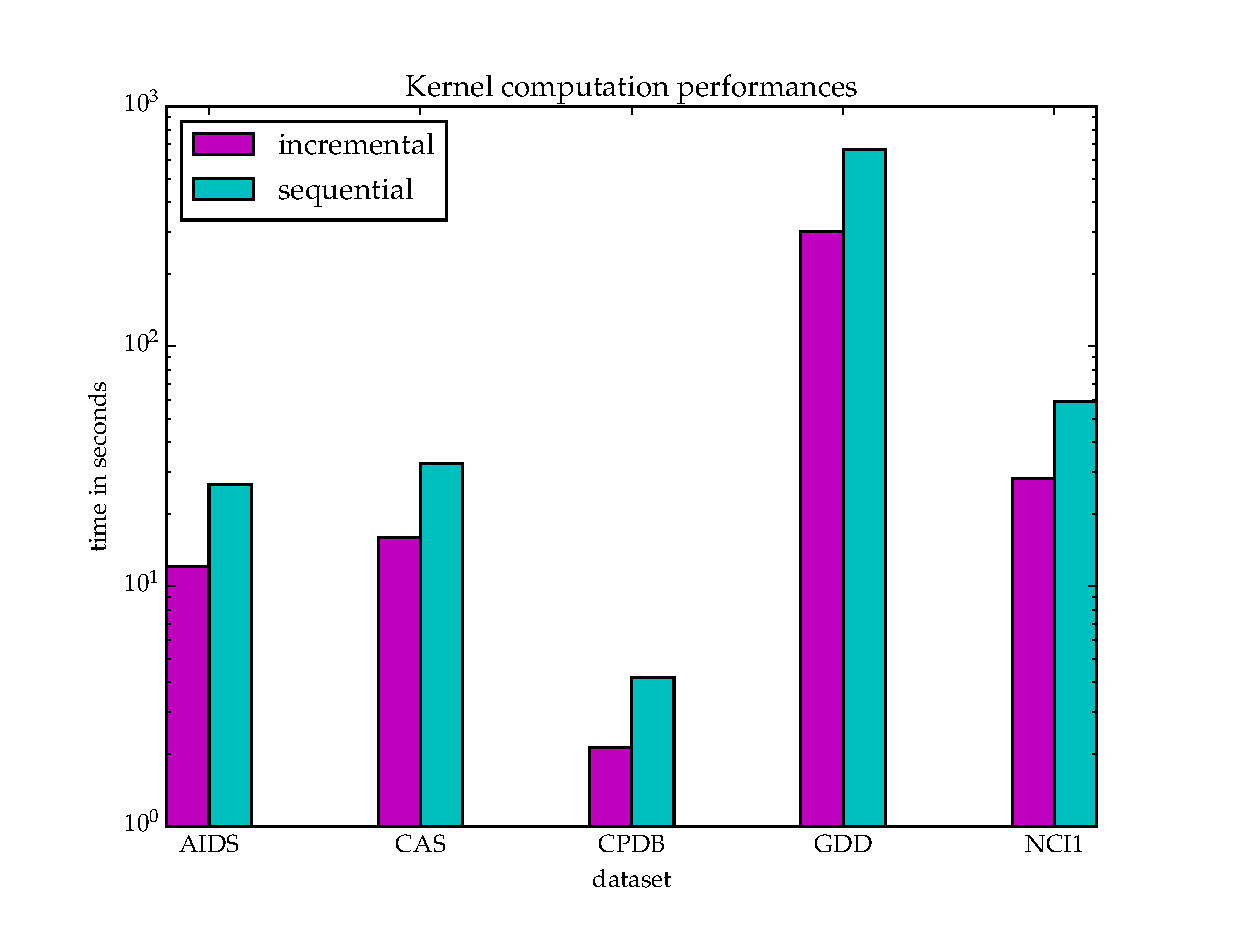
\includegraphics[scale=0.5]{Figures/kernel_times_log}
    \caption{Times in seconds required to compute the kernels $ODDK_{ST}$ and 
    $TCK_{ST}$ incrementally and sequentially on a selection of datasets. Time
    scale is logarithmic for the sake of presentation.}
    \label{fig:times}
\end{figure}

The plot in figure~\ref{fig:times} shows the relation between the computation times
on a variety of datasets, see Section~\ref{subsec:datasets} for further details on
the composition of each dataset.

%----------------------------------------------------------------------------------------

% vim: spell spelllang=en_gb
